\documentclass[11pt]{article}
\usepackage{acl}
\usepackage{times}
\usepackage{latexsym}
\usepackage[T1]{fontenc}
\usepackage[utf8]{inputenc}
\usepackage{microtype}
\usepackage{graphicx}
\graphicspath{{./figs}}

\title{Does N-gram Conditional Memory Help Small Dense Transformers?
A Minimal Replication of DeepSeek's Engram}

\author{
	Khoa Cao \and Kohki Hatori \and Haoran Su \\
    Boston University \\
	\texttt{kcao@bu.edu, khatori@bu.edu, suhr08@bu.edu}
}

\begin{document}
\maketitle

% -----------------------------------------------------------------------------
% Midway report specs from CS505 final project handout:
% - 2--4 pages, ACL format
% - Written like a short research paper
% - Include: Abstract, Introduction, Progress, Project Plan, References
% - Abstract < 250 words
% - For empirical projects: Methods, Experiments, Results
% - For survey projects: Overview/Taxonomy, Technical Summaries, Discussion
% -----------------------------------------------------------------------------

\begin{abstract}
Large language models must balance compositional reasoning with efficient retrieval of fixed, local patterns such as multi-token entities and formulaic phrases. DeepSeek's Engram introduces conditional n-gram memory for this purpose, but reported gains are entangled with large-scale MoE training and architectural changes, making it unclear whether conditional memory alone helps smaller dense models. 
We study this question by implementing an end-to-end PyTorch replication on WikiText-103 using a GPT-2 style 85M-parameter decoder-only backbone \cite{radford2019language}. Our framework includes three matched variants: a dense baseline, a parameter-control model with extra dense adapters, and Engram-augmented models with either frozen or learnable gates, all trained under the same tokenizer, data pipeline, optimization schedule, and evaluation protocol. 
In initial runs, the dense baseline currently achieves the best validation perplexity (28.72), while Engram variants underperform on final perplexity (34.95 and 35.88 for learnable and frozen gates, respectively). However, both Engram variants converge substantially faster (about 34k steps) than the dense baseline (53.7k steps), suggesting a possible optimization or parameter-efficiency advantage despite weaker end perplexity in this setting. 
Before the final report, we will complete remaining control runs, run test-set evaluation for all variants, and perform diagnostic analyses on various language modeling tasks and visualize gate activations to isolate when conditional memory is beneficial to small dense transformers. Code available at \url{https://github.com/koacow/deepseek-engram-lm}.
\end{abstract}

\section{Introduction}
% Required by spec:
% - Give a concrete example and technical definition of the problem.
% - Explain why the problem is interesting/important.
% - Explain why the problem is hard and how obvious solutions fail.

\subsection{Why This Problem Matters}
% Scientific relevance and/or real-world impact.

Language modeling involves two qualitatively different subproblems: reasoning about the compositional structure of language and knowledge retrieval.
While compositional reasoning requires deep, dynamic computation — something standard transformer architectures are well-suited for — knowledge retrieval — multi-
token named entities, formulaic phrases, and other local n-gram regularities, is often more static. 
Classical n-gram models capture these patterns cheaply via lookup tables, but modern neural LMs discard them
entirely, forcing the network to reconstruct static associations through layers of attention and feed-forward computation.

DeepSeek's Engram paper \cite{cheng2026engram} proposes conditional memory as a complementary axis of model capacity: 
a trainable, hash-addressed n-gram embedding module that is inserted into specific transformer layers and trained jointly from scratch with the backbone.
It relies on sparse lookup operations to retrieve static embeddings for fixed-knowledge. The Engram module, specifically, is conditional memory grounded in
the classic n-gram structure but with modern additions such as tokenizer compression, multi-head hashing, and contextual gating.

The paper found that an Engram model, when compared to an equally sized dense transformer, achieved better performance on knowledge retrieval, general reasoning, 
and code/math tasks. However, the gains reported coincided with other architectural innovations such as manifold-constrained hyper-connections - Deepseek's modified constrained residual connection structure that consists of multiple parallel branches that 
fixes the instability problem of unconstrained hyper-connections \cite{xie2026mhcmanifoldconstrainedhyperconnections}, MoE routing, 
and a massive scale (27B parameters). It is thus unclear how much of the improvement can be attributed to the Engram module itself, and whether it would still be effective in smaller models.

This project aims to answer the question: Does n-gram conditional memory alone benefit a compact, standard dense transformer trained from scratch? 

\subsection{Why It Is Difficult}
% Describe failure modes of simple baseline(s) or obvious approaches.

Answering this question comes with a few engineering challenges. First, we must adapt forward pass demonstration in the public Engram repository to a full training loop for a 85M parameter GPT-2 style transformer. We also 
simplify the multi-branch residual stream, which prior work has shown to be a key driver of Engram's performance \cite{larsson2017fractalnet,szegedy2014goingdeeperconvolutions,xie2026mhcmanifoldconstrainedhyperconnections,zhu2025hyperconnections}, to a single branch. Finally,
we must reproduce the paper's tokenizer compression technique, which was adapted to the DeepSeek 128k tokenizer, to work for GPT-2's 50k tokenizer.

\subsection{Problem Setup and Example}
% Define task clearly (input/output, objective).
% Provide one concrete motivating example.

We train four models: a 85M parameter GPT-2 style transformer \cite{radford2019language}, a transformer with an extra dense MLP layer to match the later Engram models' parameter count,
a transformer with an Engram module with gating fixed at $\alpha_t = 0.5$ (removing the contextual gating), and a transformer with an Engram module with learnable gating. 
We train and evaluate the perplexity of these models on the WikiText-103 dataset \cite{merity2016pointer}.

The key comparison is between the second and fourth models: if the Engram module provides a unique benefit beyond just adding more parameters, then we should see a significant perplexity improvement in the fourth model compared to the second, even though they have the same parameter count.
After an initial training run, we find that the ParamsControlLM achieved the lowest training loss and validation perplexity at 3.1979 and 28.1504, respectively.
It is followed by the BaselineLM (3.2117 training loss, 28.7229 validation PPL), the EngramLM with learnable gate (3.3184 training loss, 34.9481 validation PPL), and the EngramLM with frozen gate (3.2651 training loss, 35.8792 validation PPL).
Even though the Engram models performed slightly worse than the dense baseline, they train signinificantly faster, with the learnable-gate variant converging in 34{,}000 steps and the frozen-gate variant converging in 34{,}200 steps, compared to 53{,}700 steps for the dense baseline and 52{,}500 steps for the parameter-control baseline.
This suggests that the Engram module may provide be more parameter-efficient for learning, even if it does not achieve the lowest perplexity in this setting. We will perform further analyses to understand the training dynamics and the contribution of the Engram module.

\section{Methods and Experiments}
% Keep this section if your project is empirical.
% If your project is a survey, replace this entire section with Section 2A below.
We have implemented an end-to-end training pipeline in PyTorch, including dataset ingestion, three model variants, optimization with warmup/decay scheduling, periodic validation, and checkpoint resume/save logic.
The current codebase supports direct comparison between dense and memory-augmented architectures under matched training conditions.

\subsection{Methods}
% Describe implemented method with enough detail for reimplementation.
% Include model architecture, algorithms, and any equations/figures needed.
% Mention what is already implemented vs. in progress.
Our implementation consists of (i) a shared GPT-2 style decoder-only backbone, (ii) model-specific adapter modules, and (iii) a unified causal language-model training objective \cite{radford2019language}.

\paragraph{Data ingestion and preprocessing.}
We load \texttt{wikitext-103-raw-v1} via HuggingFace \texttt{datasets} and tokenize with the GPT-2 tokenizer (\texttt{AutoTokenizer}, fast mode).
If no pad token is defined, we set pad to EOS for consistent batching.
After tokenization, we concatenate token streams within each split and chunk into fixed-length sequences of length 512.
Each chunk is used as \texttt{input\_ids}, and \texttt{labels} are copied from \texttt{input\_ids}.
The actual next-token shift is applied inside the loss function.

\paragraph{Backbone architecture.}
All model variants share the same backbone defined in \texttt{modeling.py}:
token and positional embeddings, 12 transformer blocks, RMSNorm pre-normalization, causal multi-head self-attention, and a 2-layer GELU MLP in each block.
The language-model head is weight-tied with token embeddings.
The training loss is standard teacher-forced causal cross-entropy, implemented by aligning $\texttt{logits}[:, :-1]$ with $\texttt{labels}[:, 1:]$.

\paragraph{Comparing model variants.}
We currently train three variants from the same base configuration:
\begin{itemize}
	\item \textbf{BaselineLM}: shared dense transformer backbone only.
	\item \textbf{ParamsControlLM}: adds a residual \texttt{ControlAdapter} (RMSNorm $\rightarrow$ up-projection $\rightarrow$ GELU $\rightarrow$ down-projection) at selected layers to provide a parameter-count control condition.
	\item \textbf{EngramLM}: adds an \texttt{EngramAdapter} at the same selected layers.
\end{itemize}

\paragraph{Engram adapter implementation.}
Our Engram module uses hash-addressed n-gram memory with orders $(2,3)$ inserted at layers $(2,6)$.
For each layer/order/head, we allocate a separate embedding table with prime table sizes to reduce collisions.
Given token IDs, we construct shifted n-gram contexts, compute XOR-style hash mixes with layer-specific odd multipliers, and retrieve per-head memory embeddings.
Retrieved memory is concatenated and projected to key/value vectors.
The query comes from current hidden states.
A scalar gate per token is either learnable ($\sigma((q\cdot k)/\sqrt{d})$) or fixed at 0.5 for ablation.
The final memory update includes a depthwise causal short-convolution branch and is added residually to the block output.

\paragraph{Training loop status.}
We have implemented a full optimizer-step loop with gradient accumulation, gradient clipping, scheduler stepping, periodic validation perplexity, CSV logging, checkpoint save/resume, and final test-set perplexity export.
This infrastructure is complete and currently used for all model variants.


\subsection{Experiments}
% Dataset(s): name, split details, preprocessing, and citations.
% Evaluation metrics and rationale.
% Training/inference setup: key hyperparameters, compute budget, runtime.
% Baseline(s): simple and strong baselines used for comparison.
\paragraph{Dataset and splits.}
All experiments use WikiText-103 with the standard train/validation/test splits provided by HuggingFace \cite{merity2016pointer}.
Preprocessing follows the fixed-length chunking procedure described above (block size 512), with no additional corpus filtering beyond tokenizer processing.

\paragraph{Evaluation metric.}
Our primary metric is perplexity (PPL), computed as $\exp(mean(L_{CE}))$ on validation and test batches.
Evaluation uses the same shifted causal objective as training.
During training, validation PPL is measured every 5{,}000 optimizer steps; final reporting includes test PPL (up to 500 test batches in the current script).

\paragraph{Training configuration.}
Current default settings are: batch size 8, gradient accumulation 4 (effective batch size 32), 100{,}000 optimizer steps, AdamW ($\texttt{lr}=3\times10^{-4}$, weight decay 0.1), linear warmup for 2{,}000 steps, cosine decay to $10^{-5}$, and gradient clipping at 1.0.
We train on CUDA when available (otherwise CPU), use deterministic seeds for Python/NumPy/PyTorch, and log step/loss/PPL/LR to per-model CSV files.
Checkpoints are saved every 10{,}000 steps and can be resumed from disk.

\paragraph{Comparison protocol.}
The active comparison includes:
\begin{itemize}
	\item \textbf{Dense baseline} (BaselineLM),
	\item \textbf{Parameter-control baseline} (ParamsControlLM), and
	\item \textbf{Engram memory model} (EngramLM), with both frozen-gate and learnable-gate settings.
\end{itemize}
All variants share tokenizer, data pipeline, sequence length, optimization schedule, and evaluation procedure to isolate effects of memory augmentation versus added dense parameters.

\section{Results}
% Present quantitative/qualitative results using tables/figures.
% Do not bury key numbers in plain text only.
% Briefly interpret trends: expected vs observed behavior.
% Include any error analysis and what it suggests to improve next.

\subsection{Pre-training results}

The results of the initial training runs are summarized in Table \ref{tab:Table1}. Figures \ref{fig:training_loss} and \ref{fig:validation_ppl} show the training loss and validation perplexity for each model variant across the training process. The ParamsControlLM achieved the lowest training loss and validation perplexity, followed by the BaselineLM, the EngramLM with learnable gate, and the EngramLM with frozen gate. 
However, the Engram models converged significantly faster than the dense baseline, suggesting that the Engram module may provide more parameter-efficient learning even if it does not achieve the lowest perplexity in this setting.
\begin{table*}[h]
\centering
\begin{tabular}{|l|c|c|c|}
\hline
Model Variant & Lowest Training Loss & Lowest Validation PPL & Steps to Converge \\
\hline
BaselineLM & 3.2117 & 28.7229 & 53{,}700 \\
ParamsControlLM & 3.1979 & 28.1504 & 52{,}500 \\
EngramLM (Learnable Gate) & 3.3184 & 34.9481 & 34{,}000 \\
EngramLM (Frozen Gate) & 3.2651 & 35.8792 & 34{,}200 \\
\hline
\end{tabular}
\caption{Training loss, validation perplexity, and convergence steps for each model variant.}
\label{tab:Table1}
\end{table*}

\begin{figure}[h]
\centering
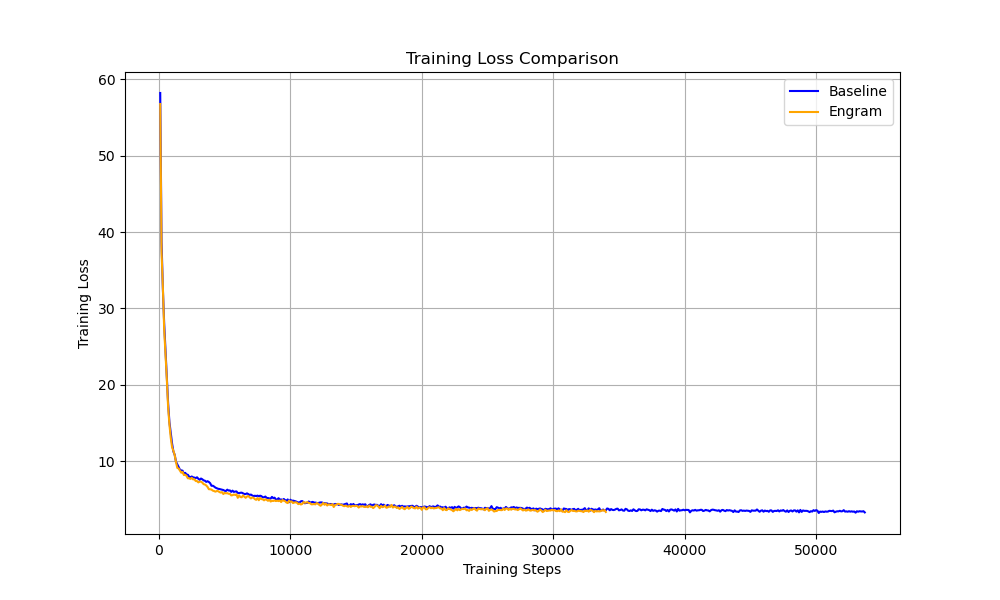
\includegraphics[width=0.4\textwidth]{training_loss_comparison.png}
\caption{Training loss across steps for each model variant.}
\label{fig:training_loss}
\end{figure}

\begin{figure}[h]
\centering
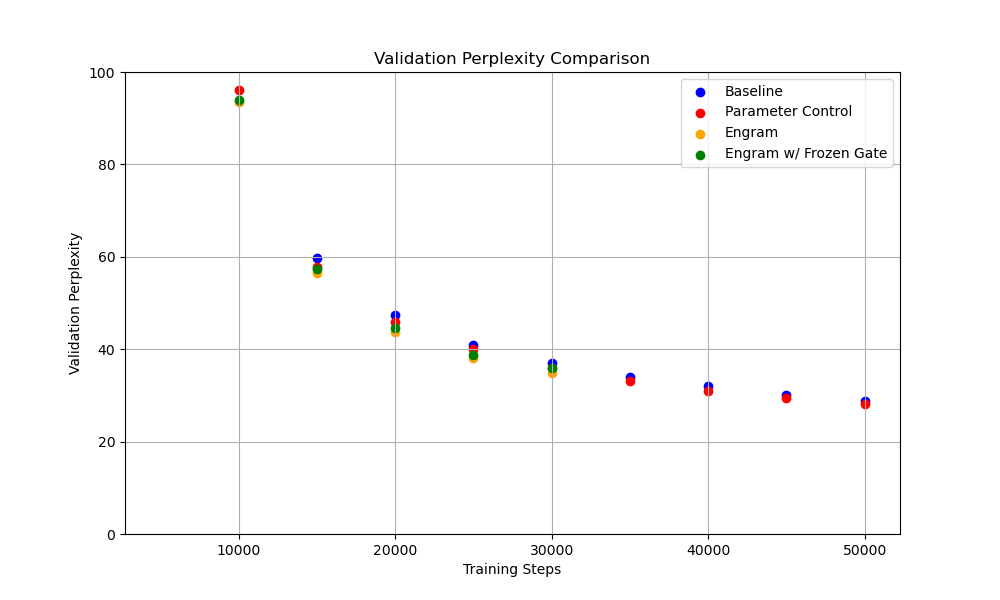
\includegraphics[width=0.4\textwidth]{validation_perplexity_comparison.png}
\caption{Validation perplexity across steps for each model variant.}
\label{fig:validation_ppl}
\end{figure}	

With that said, the current results are suprising given that the Engram module is designed to enhance retrieval of fixed n-gram patterns, which should be beneficial for language modeling, specifically for knowledge retrieval tasks.
TODO: evaluate model on test set

\subsection{Evaluating on Language Modeling Tasks}

We evaluated the ParamsControlLM and EngramLM with learnable gates on the BLiMP and MMLU benchmarks, which test for linguistic phenomena and general knowledge, respectively \cite{warstadt-etal-2020-blimp-benchmark,hendrycks2021measuringmassivemultitasklanguage}.
The results are summarized in Table \ref{tab:Table2}.
TODO: add results and analysis

\subsection{Visualizing Gate Activations}
Similar to the Engram paper's analysis of the context-aware gating mechanism, we visualize the gate activations across tokens and Engram layers (2 and 6)
for the EngramLM with learnable gates, shown in Figures~\ref{fig:engram_gating_heatmap} and~\ref{fig:engram_gating_line_plot}.
We evaluate on the same sentences used in the Engram paper, replacing the latter two with English sentences containing multi-token named entities and formulaic phrases.

From the heatmaps in Figure~\ref{fig:engram_gating_heatmap}, several patterns emerge.
First, the two layers exhibit qualitatively different gating behavior: Layer 2 produces relatively uniform, moderate activations across most token positions, whereas Layer 6 displays sharper, more selective gating with higher contrast between suppressed and active tokens.
This suggests a hierarchical division of labor, in which early layers pass content through broadly and deeper layers apply more targeted suppression based on accumulated contextual information.

Second, within Layer 6, activations tend to peak at sentence-initial tokens and decay toward the right, indicating a positional bias in the gating signal that may reflect the module's sensitivity to how much context has been accumulated at each position.

Third, and most notably, gate activations are highest at tokens that complete retrievable n-gram patterns.
For example, activations peak at ``Great'' in ``Alexander the Great'' and ``way'' in ``by the way'', both of which are plausible high-frequency n-grams in the WikiText-103 training data.
Conversely, multi-token named entities such as ``Princess Diana'' and ``the President of the United States'' exhibit strong suppression at Layer 6, suggesting that the module learns to inhibit memory retrieval for spans that are unlikely to be resolved by static n-gram lookup alone.

Overall, these visualizations suggest that even at a substantially smaller model and dataset scale, the Engram module learns to conditionally gate n-gram memory retrieval based on contextual cues.
While these results are broadly consistent with the findings reported in the Engram paper, the gating patterns are less sharp and consistent than those observed in the original work, which we attribute to the limited capacity of a smaller model and corpus to learn precise memory retrieval patterns.

\begin{figure}[h]
\centering
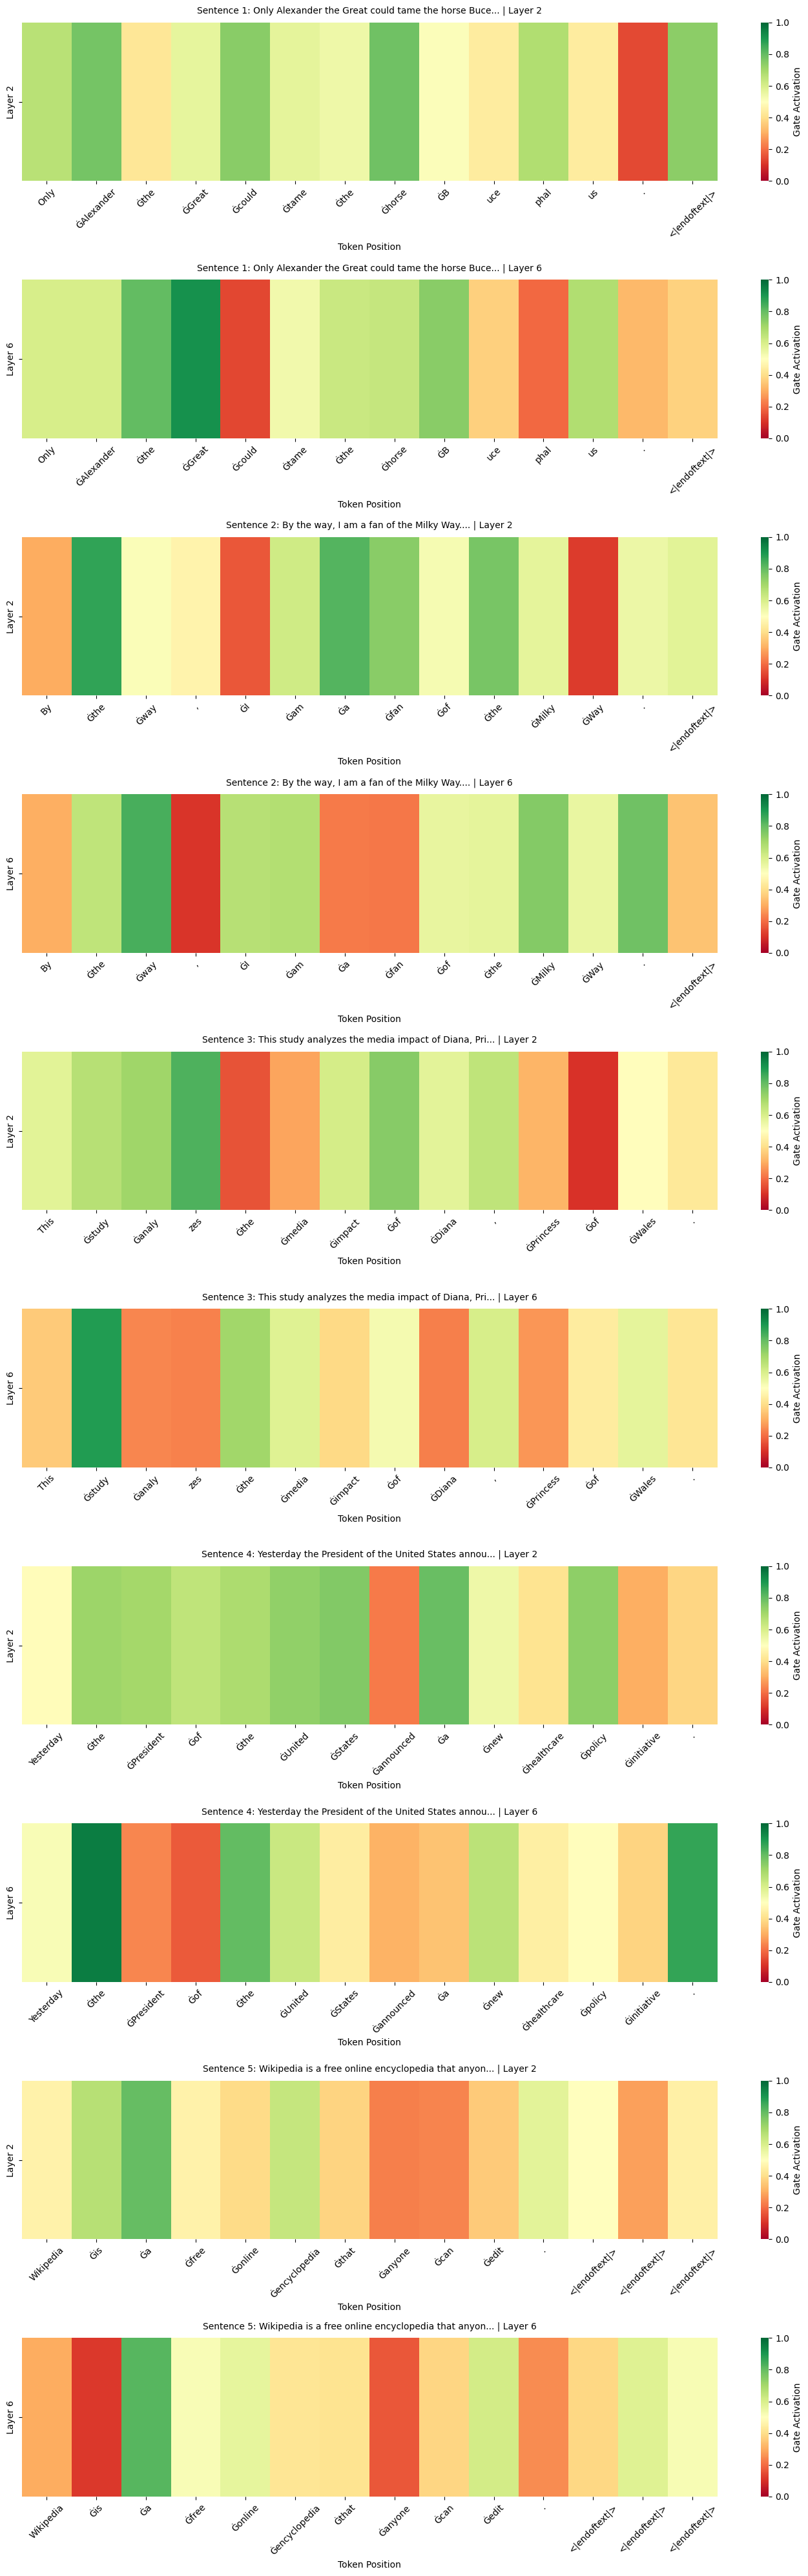
\includegraphics[width=0.5\textwidth]{engram_gating_heatmap.png}
\caption{Heatmap of Engram gate activations across tokens and layers.}
\label{fig:engram_gating_heatmap}
\end{figure}

\begin{figure}[h]
\centering
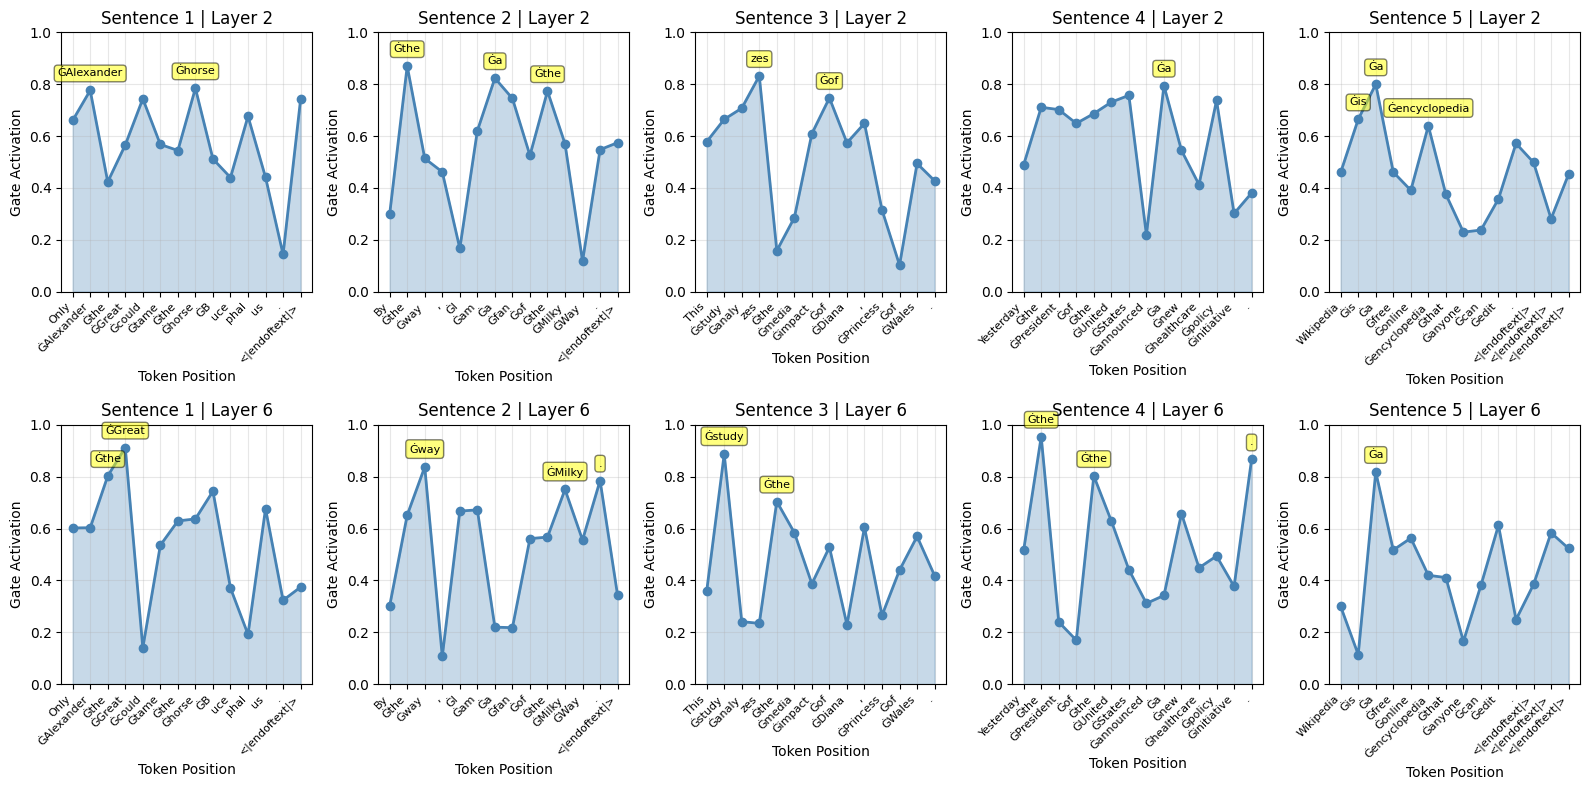
\includegraphics[width=0.5\textwidth]{engram_gating_line_plot.png}
\caption{Line plot of Engram gate activations across tokens and layers.}
\label{fig:engram_gating_line_plot}
\end{figure}

\section{Conclusion and Future Work}

% Use BibTeX if possible.
% Empirical project midway target: >= 3 references (model, dataset, related methods).
% Survey project midway target: 3--5 references per taxonomy category,
% and ideally 10--15 total by midway stage.

\bibliography{refs}
\end{document}
